\documentclass[a4paper,14pt]{extarticle}
\usepackage[left=2.5cm, right=1.5cm, vmargin=2.5cm]{geometry}
\usepackage[utf8]{inputenc}
\usepackage[T2A]{fontenc}
\usepackage[russian]{babel}
\usepackage{graphicx}
\graphicspath{{pictures/}}
\usepackage{caption}
\usepackage{subcaption}
\usepackage{indentfirst}
\setlength\parindent{5ex}
\usepackage{fancyhdr}	
\usepackage{booktabs}
\usepackage{siunitx} 
\usepackage{pgfplotstable}
\usepackage{amsmath}
\usepackage{autonum}
\usepackage{amsfonts}
\DeclareMathOperator{\sign}{sgn}
\newcommand{\gt}{\textgreater} % знак больше
\newcommand{\lt}{\textless}       % знак меньше
\DeclareGraphicsExtensions{.pdf,.png,.jpg}
\pagestyle{fancy}
\fancyhf{}
\rhead{\thepage}
\renewcommand{\headrulewidth}{0pt}

\fancypagestyle{plain}{ 
	\fancyhf{}
	\rhead{\thepage}}

\author{Никитин Илья}

\title{Отчет по лабораторной работе №2: "Масс-спектроскопия"}
\date{\today}

\begin{document}
	
	\maketitle
	\tableofcontents

	\section{Задачи}
		Проанализировать состав воздуха и других газов при помощи \\ масс-спектрометра. 
	\section{Оборудование}
		\begin{itemize}
			\item Масс-спектрометр SRS RGA-200
			\item Компьютер с предустановленным программным обеспечением для масс-спектрометра SRS RGA-200
			\item Манометр Pfeiffer TPR281
			\item Некоторое количество гелия и углекислого газа
			\item Откачной пост Pfeiffer Vacuum HiCube 80 Eco
			\item Вакуумная арматура
		\end{itemize}
	\section{Теория}
		\subsection{Масс-спектроскопия}
			Масс-спектрометрия — метод исследования и идентификации вещества, позволяющий определять концентрацию различных компонентов в нём (изотопный, элементный или химический состав). Основой для измерения служит ионизация компонентов, позволяющая физически различать компоненты на основе характеризующего их отношения массы к заряду и, измеряя интенсивность ионного тока, производить отдельный подсчёт доли каждого из компонентов (получать масс-спектр вещества).
		\subsection{Принцип работы и устройство масс-спектрометра}
			Конструкция масс-спектрометра включает в себя ионизатор вещества образца, ускоритель ионов, источник мощного магнитного поля и набор детекторов потока ионов.
			
			На заряженную частицу, движущуюся в магнитном поле, действует сила Лоренца, искажающая ее траекторию. Определяя разницу траекторий ионизированных атомов, движущихся в магнитном поле, можно делать выводы о соотношении массы и заряда иона.
			
			\begin{figure}[h!]
				\centering
				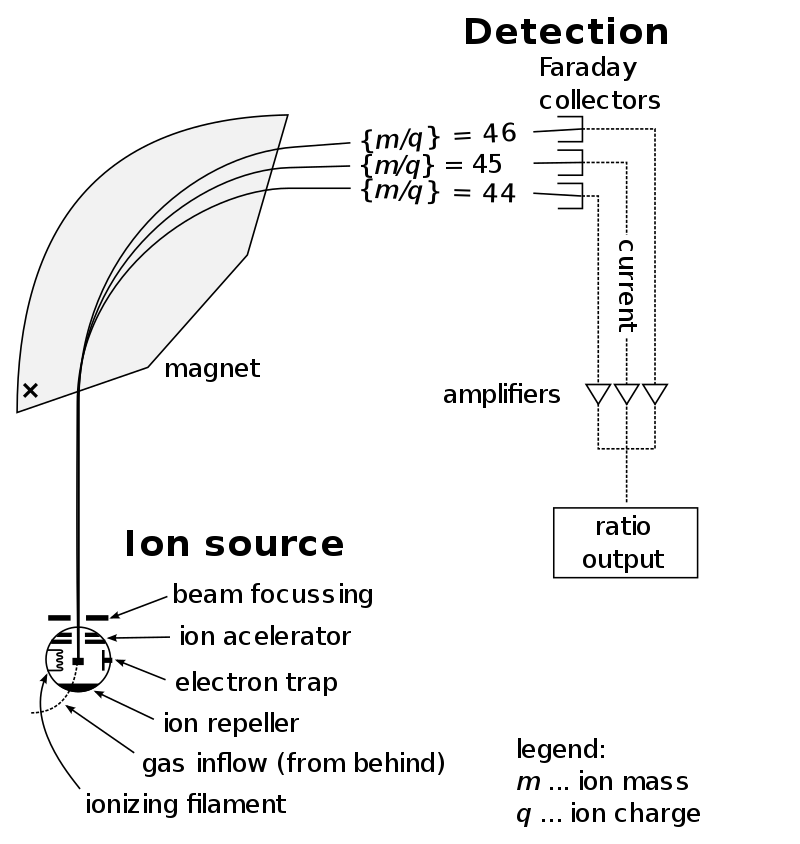
\includegraphics[width=.55\linewidth]{Lab2_1.png}
				\caption{Устройство масс-спектрометра}
				\label{fig1}
			\end{figure}
		\subsection{Спектрометр SRS RGA-200}
			Спектрометр, использующийся в работе обладает электронным принципом ионизации.
			Электронная ионизация - наиболее распространённый в масс-спектрометрии метод ионизации веществ в газовой фазе.
			
			При электронной ионизации молекулы анализируемого вещества попадают в поток электронов движущихся от эмиттирующего их катода к аноду.
			
			Электронная ионизация происходит в вакууме, чтобы предотвратить массовое образование ионов атмосферных газов, которые могут рекомбинировать с ионами анализируемого вещества и разрушать их, поэтому для работы спектрометра необходимо подключать его к вакуумному насосу. 
			
			Квадруполь представляет собой четыре параллельно и симметрично расположенных монополя (электроды круглого сечения). К электродам попарно в противоположной полярности подаётся определённая комбинация постоянного и высокочастотного напряжения ( $U_0=U+V\cos(\omega t)$, где $U$- напряжение постоянного тока, $V \cos(\omega t)$ — радиочастотная компонента).
			
			\begin{figure}[h!]
				\centering
				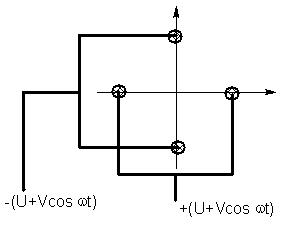
\includegraphics[width=.55\linewidth]{Lab2_2.jpg}
				\caption{Устройство масс-спектрометра}
				\label{fig2}
			\end{figure}
		
			Под действием небольшого ускоряющего напряжения (10-20 В) ионы влетают параллельно осям стержней электродов. Под действием осцилирующего поля, задаваемым электродами, они начинают колебаться вдоль осей x и y. При этом амплитуда колебаний возрастает без изменения направления движения. Ионы, чьи амплитуды достигают высоких значений, нейтрализуются при столкновении с электродами. Фиксированную амплитуду приобретают только те ионы, чьи значения $m / z$ будут отвечать определенному соотношению $U / V$. Последнее позволяет им свободно перемещаться в квадруполе и быть в конечном итоге детектируемыми. Таким образом, масс-спектр регистрируется путём взаимного изменения значений величин $U$ и $V$.
			
	\section{Анализ составов воздуха и других газов}
		\subsection{Ход работы}
			В ходе работы была собрана экспериментальная установка. К масс-спектрометру с помощью вакуумной арматуры присоединялся турбомолекулярный насос, который откачивал воздух в камере до давления в $10^{-4}$ Бар. В случае с воздухом, оставалось только включить в работу масс-спектрометр. Для гелия и углекислого газа в камеру после откачки воздуха закачивались непосредственно газы и затем снова откачивались до нужного давления.
			\begin{figure}[h!]
				\centering
				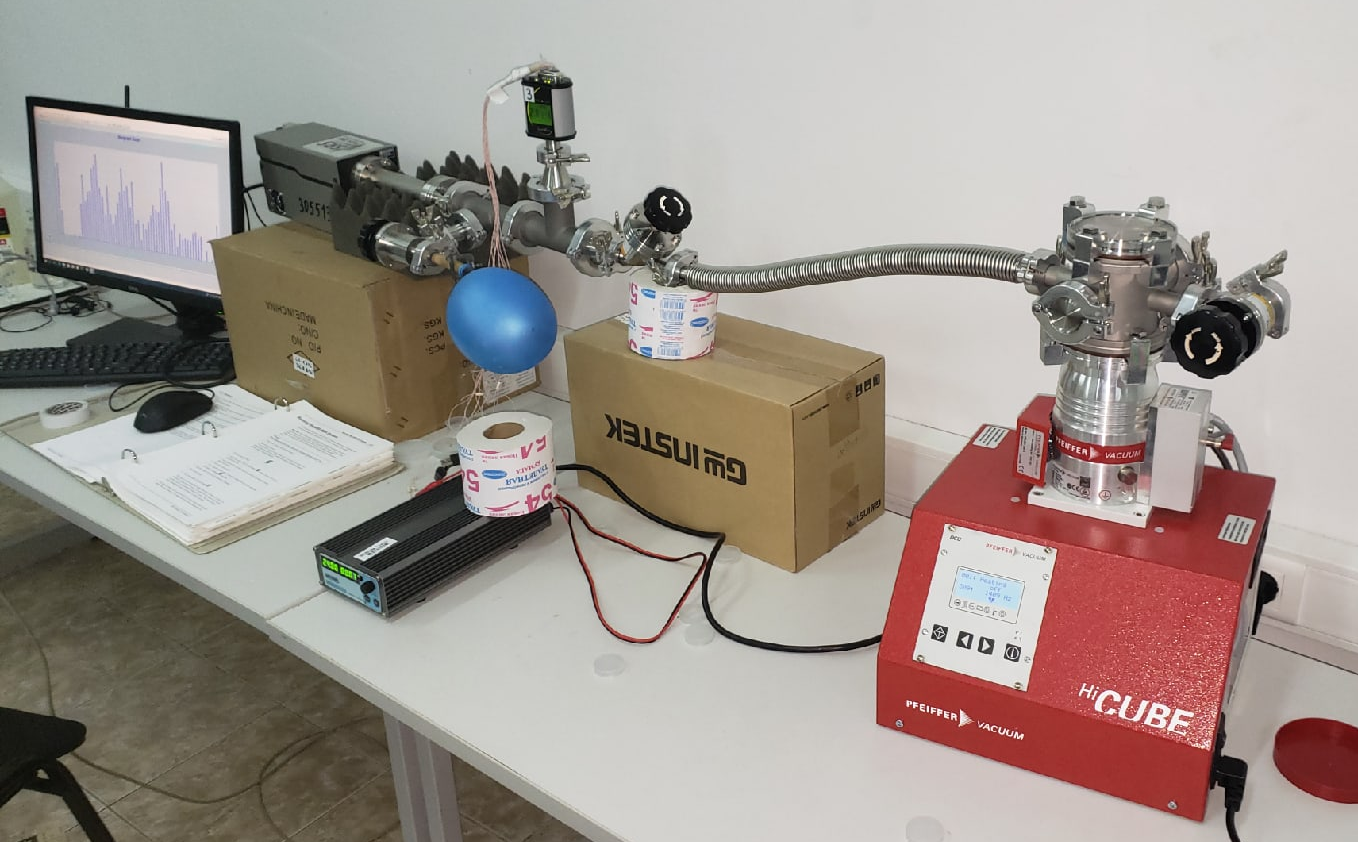
\includegraphics[width=.55\linewidth]{Lab2_3.png}
				\caption{Устройство масс-спектрометра}
				\label{fig3}
			\end{figure}
			\newpage
			
		\subsection{Обработка данных}
			\subsubsection{Воздух}
				\begin{figure}[h!]
					\centering
					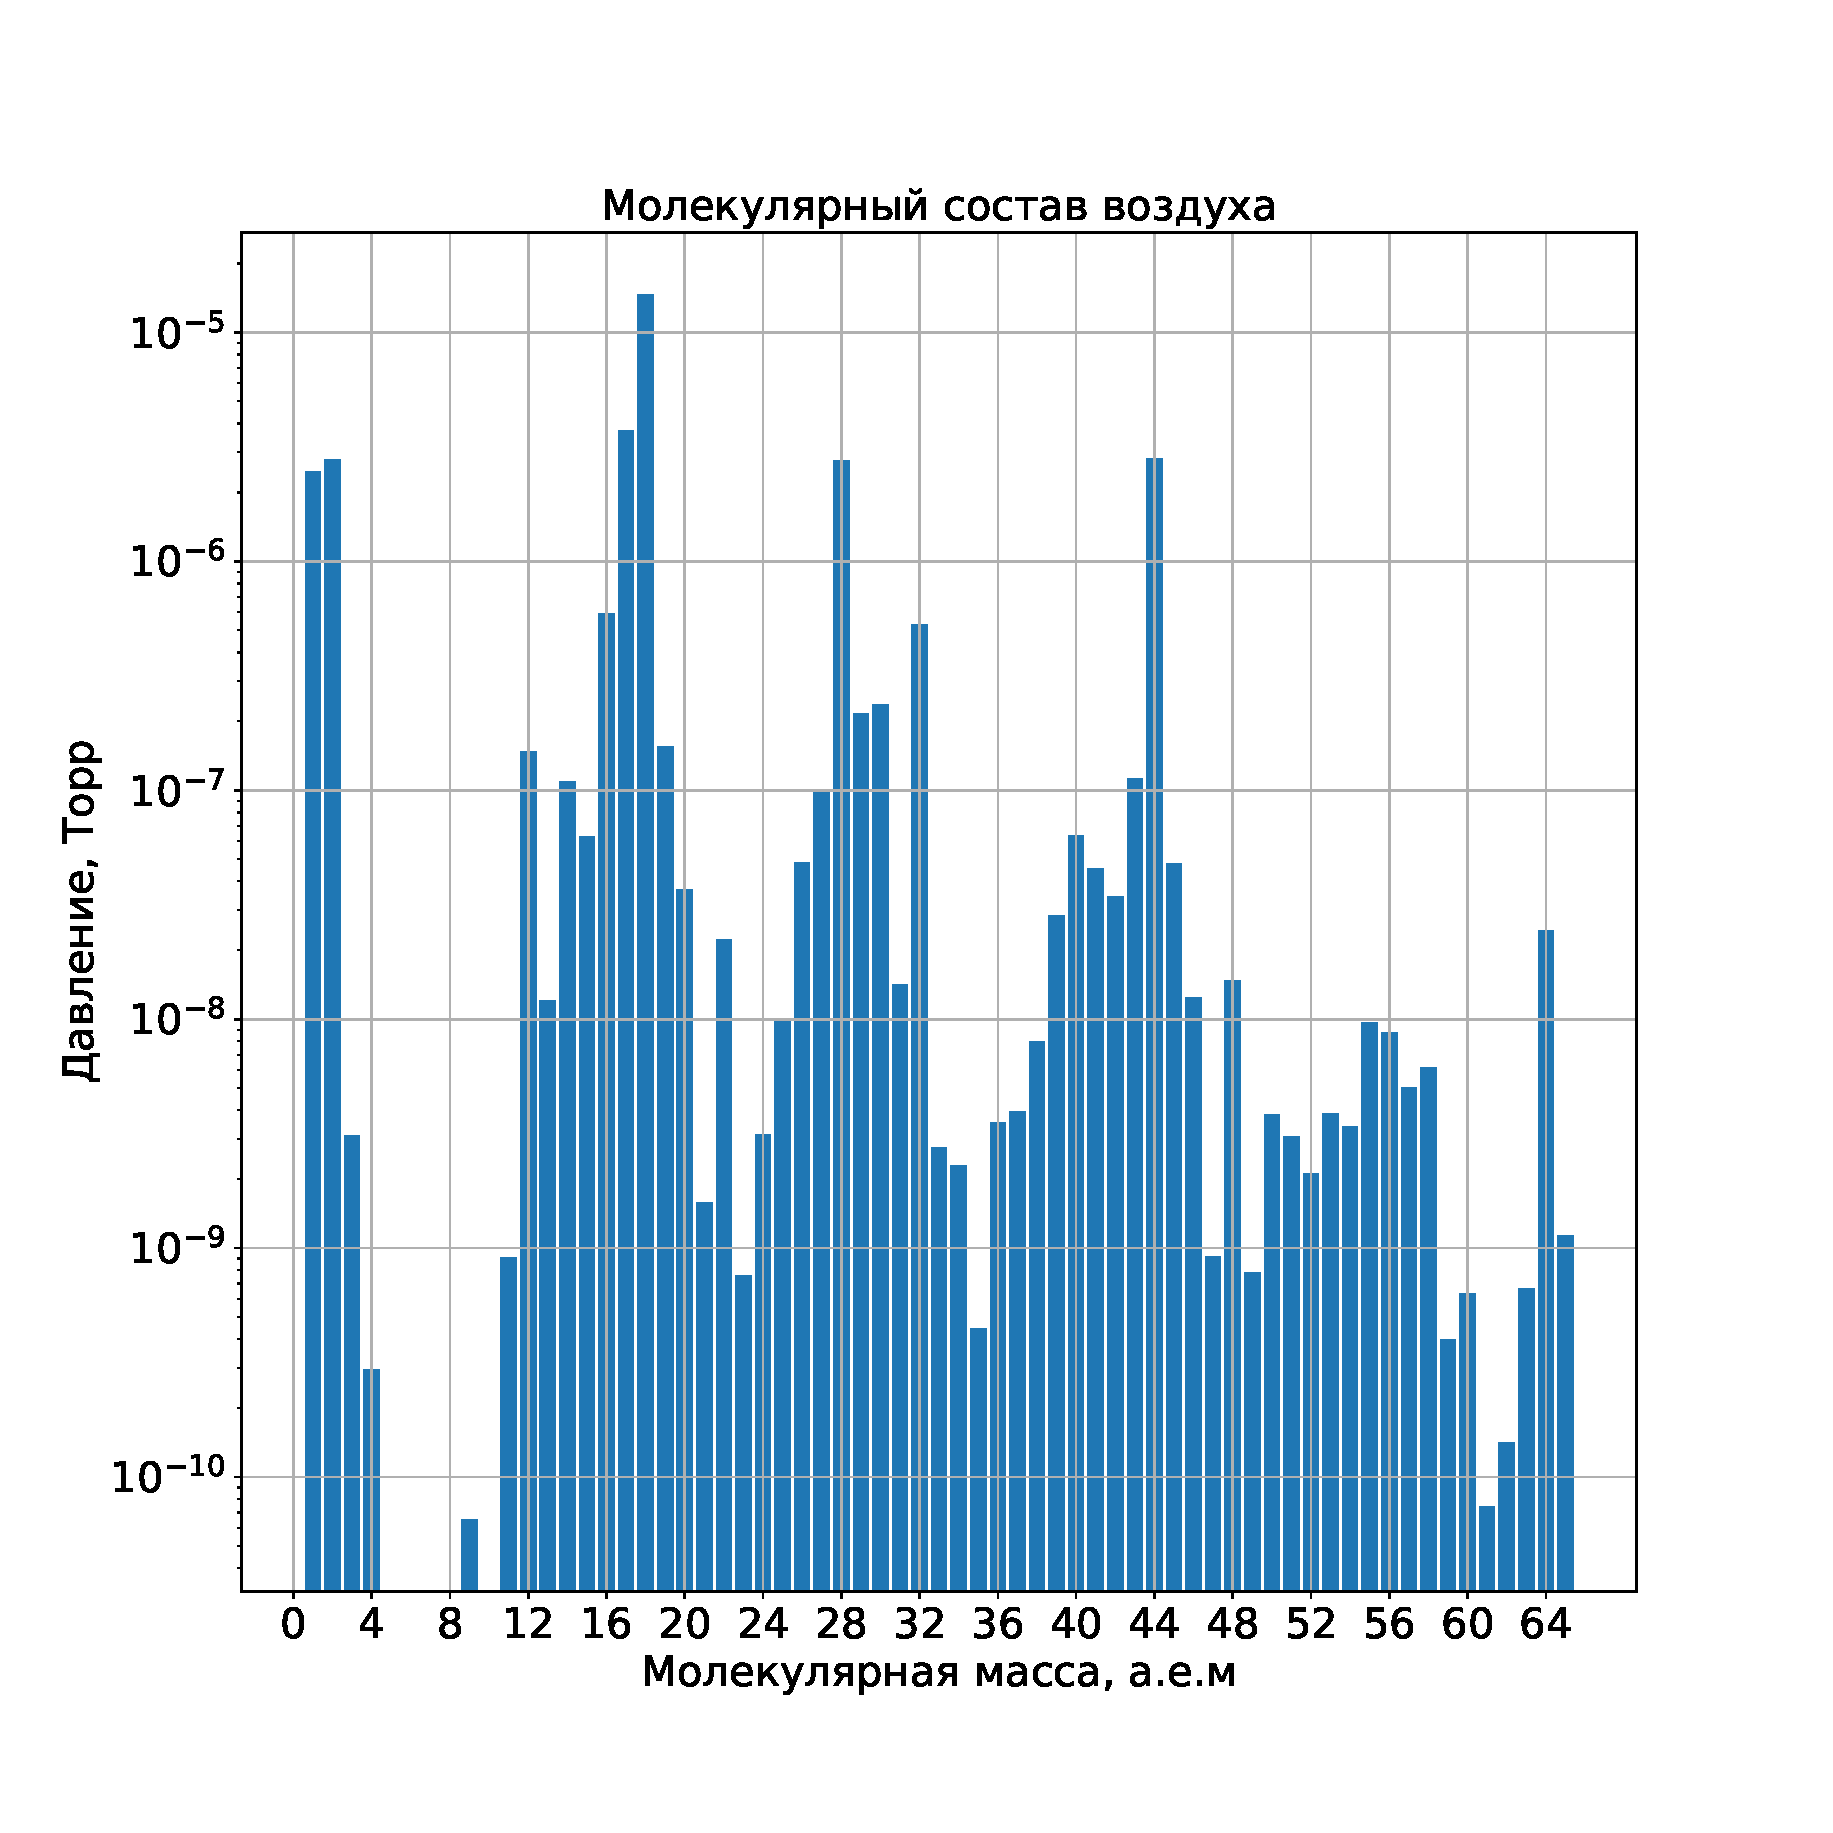
\includegraphics[width=.75\linewidth]{Lab2_1.eps}
					\caption{Масс-спектр воздуха}
					\label{fig4}
				\end{figure}
				
				На гистограмме масс-спектра воздуха можно видеть противоречивые результаты. С одной стороны, большое количество кислорода(16 а.е.м) и азота(28 а.е.м), с другой стороны огромное количество газов, которые не могут иметь соизмеримое парциальное давление с азотом и кислородом. Например, газ с атомной массой 3 (из известных мне, это мог бы быть только тритий или гелий-3, что не очень сходится со здравым смыслом).
			\subsubsection{Гелий}
				\begin{figure}[h!]
					\centering
					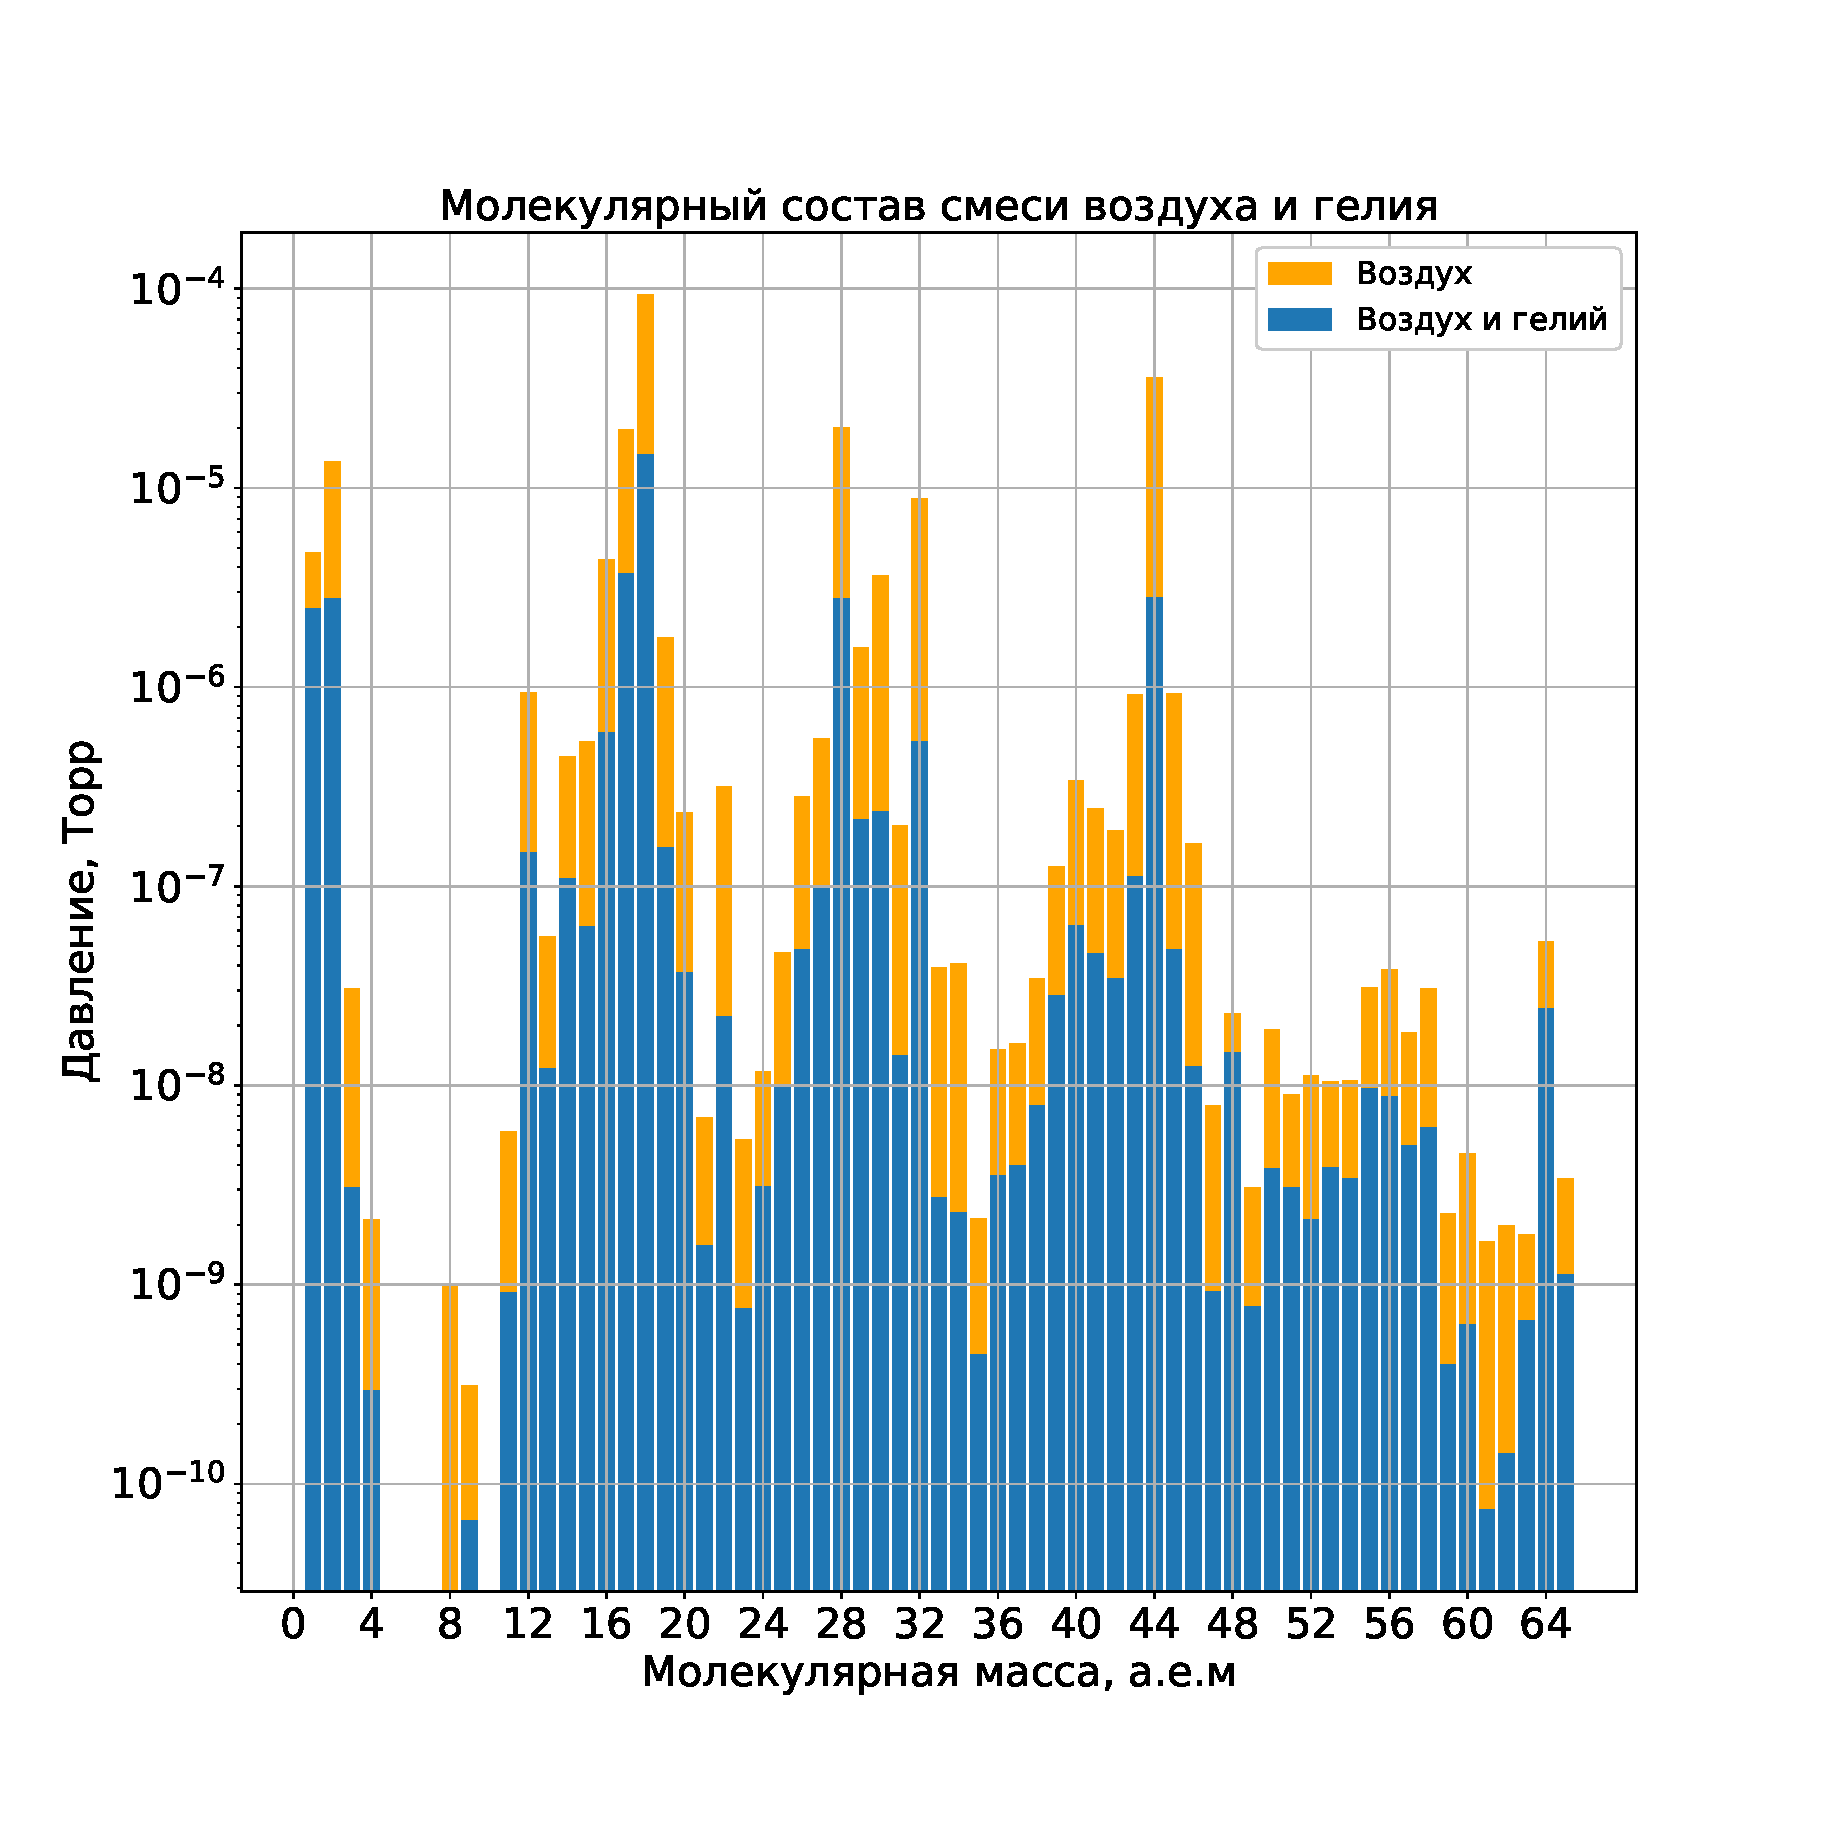
\includegraphics[width=.75\linewidth]{Lab2_3.eps}
					\caption{Масс-спектр смеси воздуха и гелия}
					\label{fig5}
				\end{figure}
				На данном графике можно заметить, что парциальное давление гелия действительно возросло на порядок, что, тем не менее, не позволило бы утверждать, что в камере находится гелий, если бы мы не знали какой газ закачиваем в камеру, так как давление остальных газов увеличилось тоже в среднем на порядок. Судя по всему, в первый раз установившееся давление в системе было ниже, чем при экспериментах с гелием (к установке добавились новые элементы, которые могли повлечь за собой образование не плотно прилегающих стыков), кроме того, гелий очень летучий
				\newpage
			\subsubsection{Углекислый газ}
				\begin{figure}[h!]
					\centering
					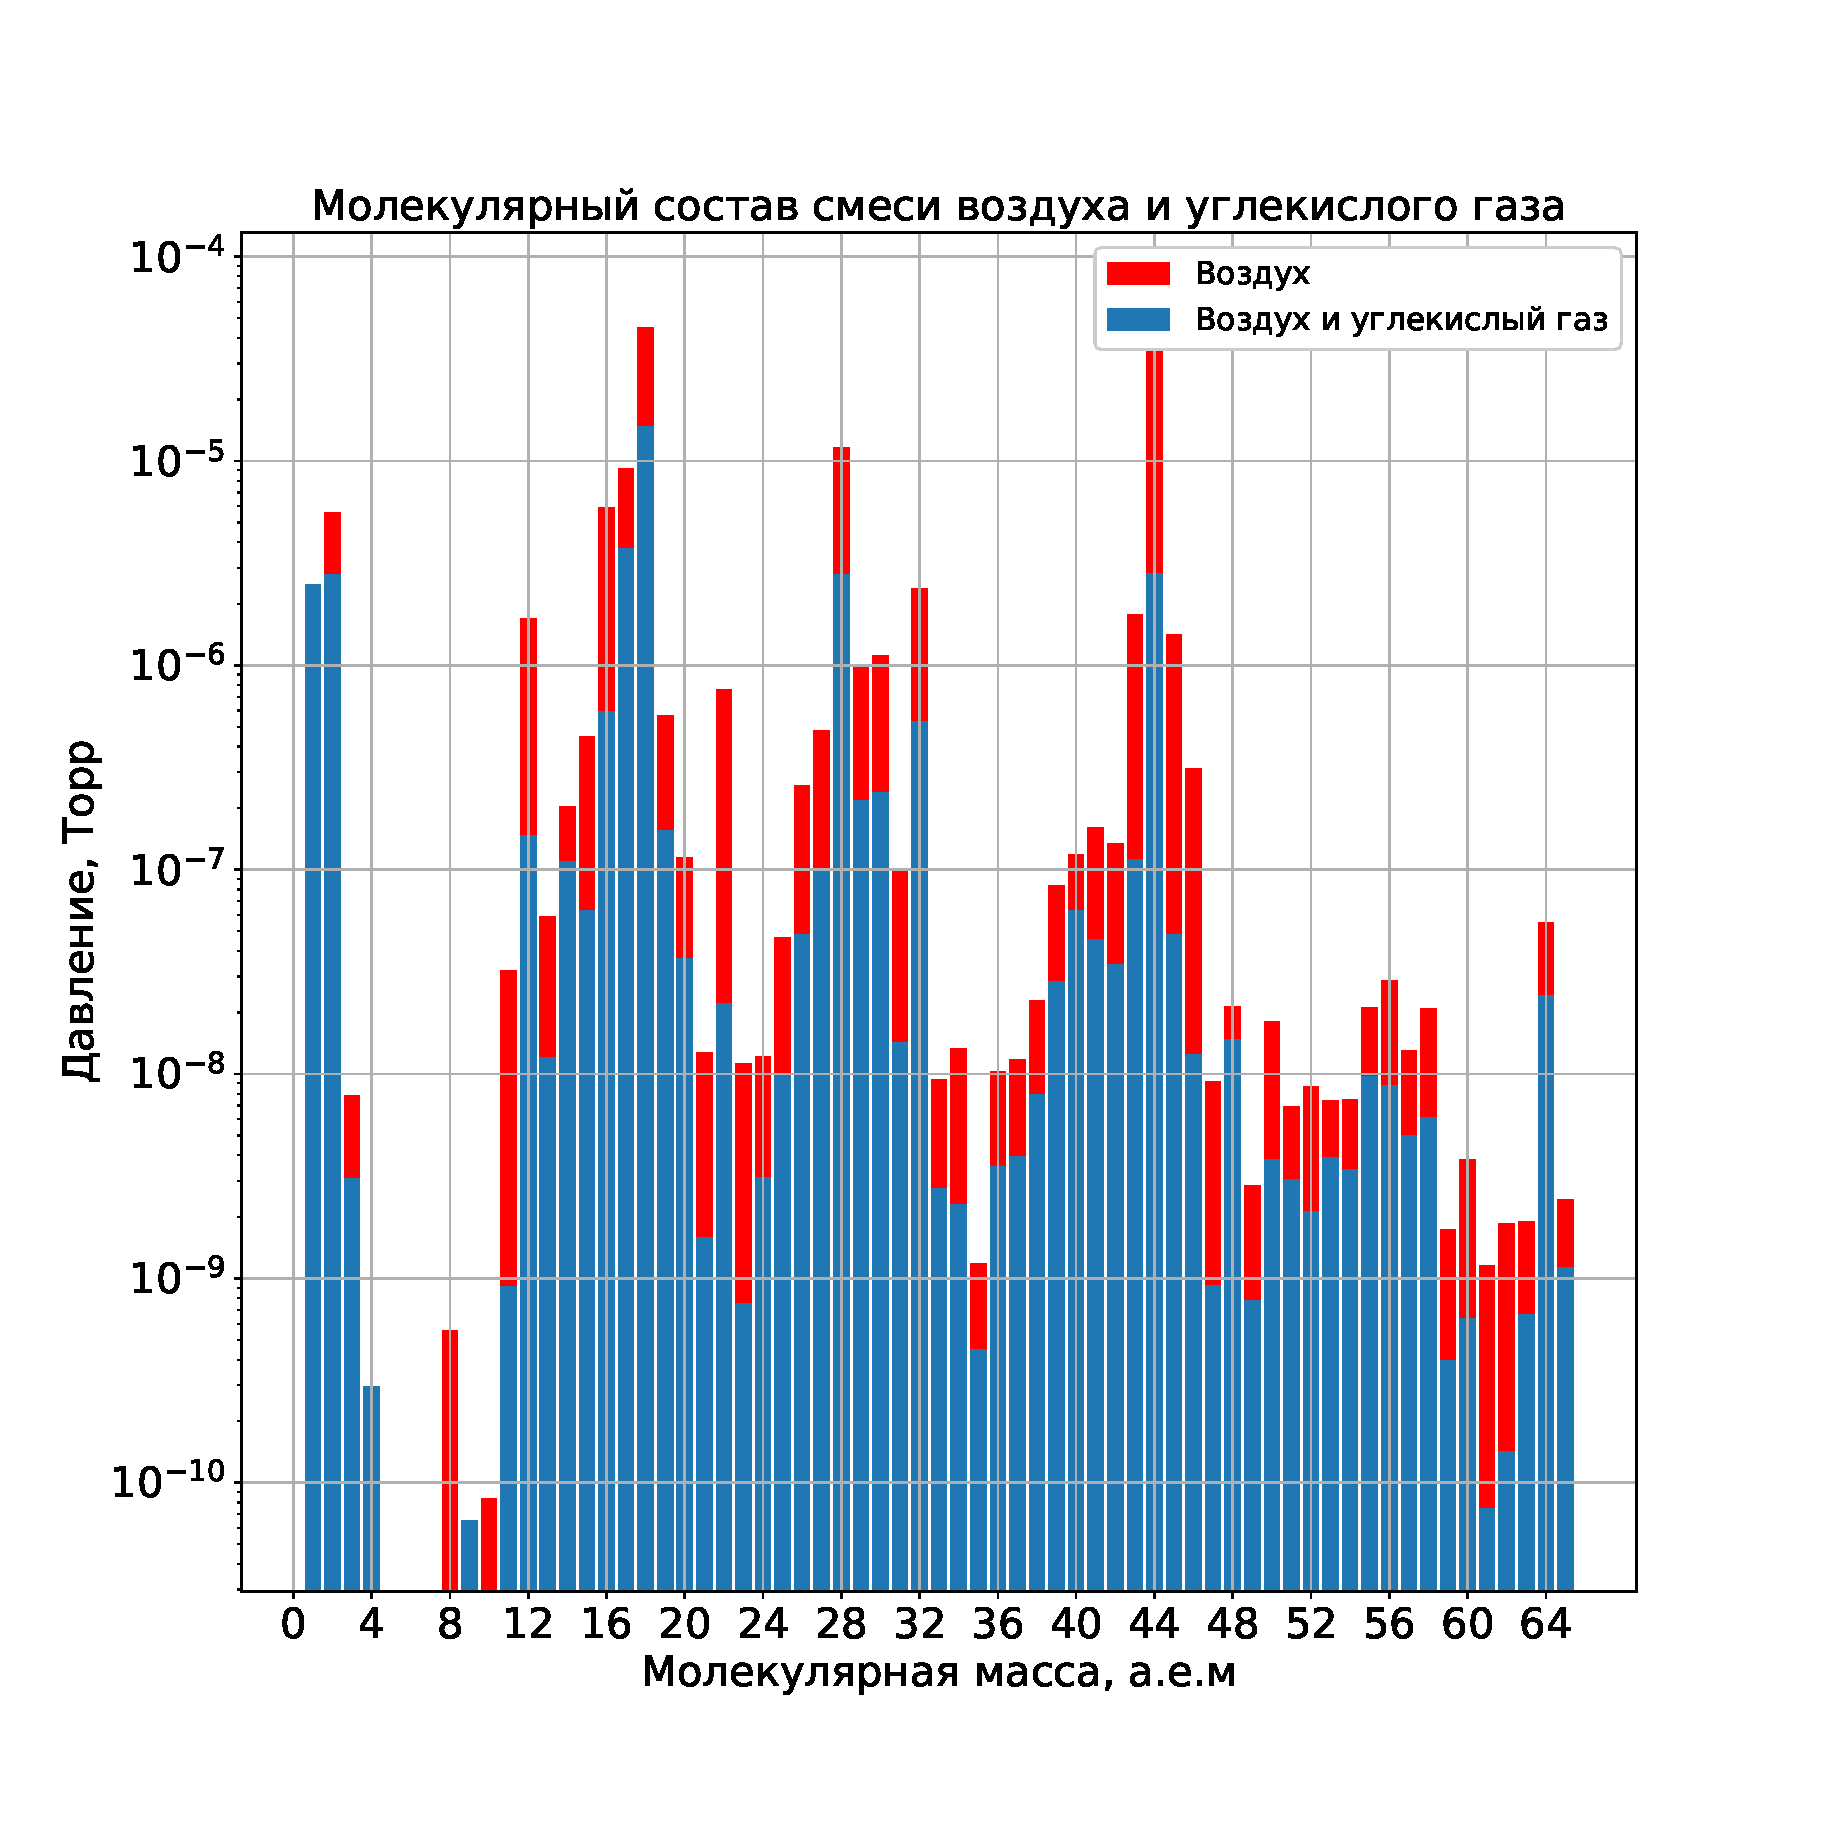
\includegraphics[width=.75\linewidth]{Lab2_2.eps}
					\caption{Масс-спектр смеси воздуха и углекислого газа}
					\label{fig6}
				\end{figure}
				Наконец, хоть какой-то адекватный результат был получен для углекислого газа. Давление всех газов в среднем возрасло на порядок по той же причине, однако давление углекислого газа изменилось несколько больше, чем давление остальных газов. Это позволило бы сказать, что в камеру был закачан углекислый газ, если бы мы этого не знали заранее.
			\subsubsection{Сравнение углекислого газа и гелия}
				\begin{figure}[h!]
					\centering
					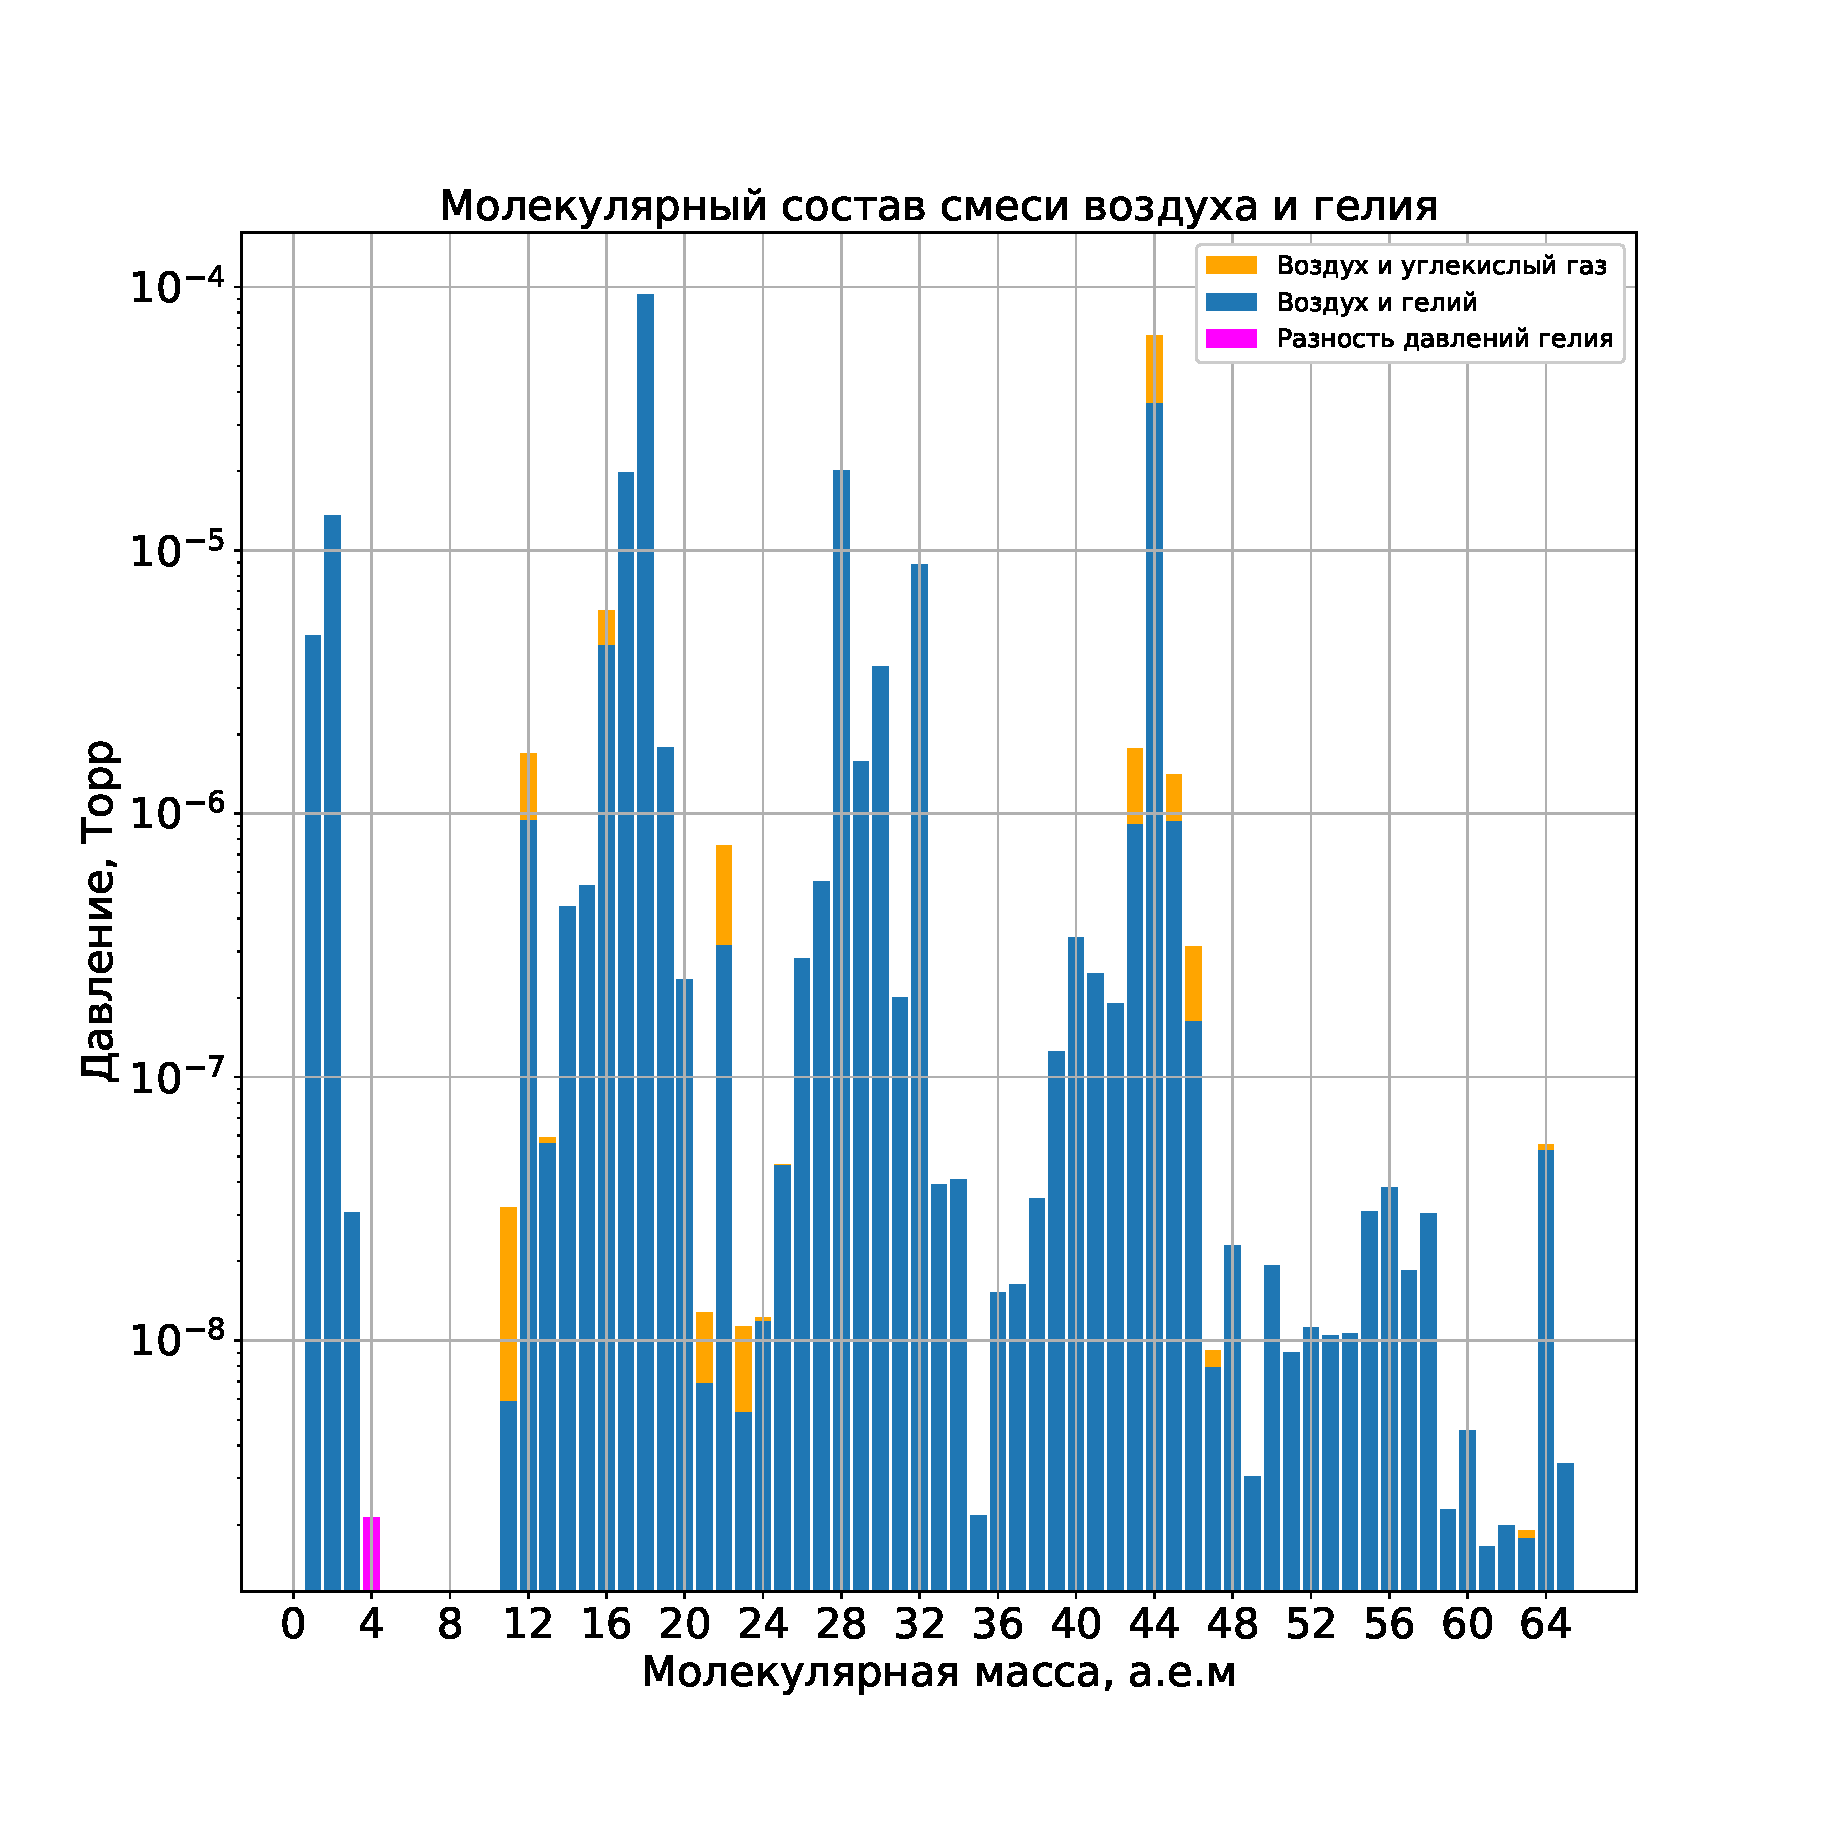
\includegraphics[width=.75\linewidth]{Lab2_4.eps}
					\caption{Масс-спектр смеси воздуха и углекислого газа в сравнении со смесью с гелием}
					\label{fig7}
				\end{figure}
				Так же я решил сделать сравнение масс-спектров смесей углекислого газа и гелия, так как они были получены при схожем давлении. Как видно из графика, разница между ними действительно есть, гелия больше в гелии, углекислого газа в углекислом газе, однако судить о точности таких данных не приходится.
	\section{Выводы}
		В ходе работы оказалось, что масс-спектрометр выдал некорректные результаты, которые имели имели только поверхностную связь с реальностью. Тем не менее, удалось пронаблюдать отличие спектра смеси из углекислого газа от спектра смеси воздуха с гелием, хоть эта разность была и не сильно отличимы от флуктуаций давлений других газов в воздухе.
\end{document}